% For tracking purposes - this is V3.1SP - APRIL 2009
\documentclass{acm_proc_article-sp}
\usepackage{graphicx}
\usepackage{subfig} % for horizontal figures
\usepackage{amsmath}
\makeatletter
\let\@copyrightspace\relax
\makeatother
\begin{document}

\title{Hierarchical Control for Aircraft Electronic Power Systems}

\numberofauthors{2}
\author{
\alignauthor
Forrest N. Iandola\\
       \affaddr{University of California, Berkeley, USA}\\
       \email{forresti@eecs.berkeley.edu}
\alignauthor
Huy Vo\\
       \affaddr{University of California, Berkeley, USA}\\
       \email{huytbvo@eecs.berkeley.edu}
}

\maketitle
\begin{abstract}
Best abstract ever
\end{abstract}

\keywords{avionics, control, optimization} 

\section{Introduction}
High-level... Increasing complexity of EPS...

We aim to design a Load Management System (LMS) for EPS that is ``smarter" in terms of several criteria.
First, always preserve safety.
After preserving safety, maximize the quality of service.
Finally, conserve fuel by using as few generators as possible.

The rest of the paper is organized as follows. (TODO)

\section{Aircraft EPS Overview}
Intro to aircraft EPS... explain the buses and generators.
Possibly show the diagram from the Honeywell patent.
Possibly show our ``cartoon" diagram of an EPS system.

\subsection{Load Shedding}
Aircraft EPS generally have two types of loads: sheddable and non-sheddable.
Examples of non-sheddable loads include navigation systems, electronic actuators, and other mission-critical devices.
Sheddable loads include the cabin lights, kitchen, and electrical outlets for passengers' laptop computers.
If an EPS power bus requires more power than the generators can provide, the LMS is responsible for disabling (shedding) some of the sheddable loads.

\section{Related Work}
\label{sec:related-work}
In typical aircraft EPS, the load management systems aim to ensure safety during unexpected system behavior [citation needed].
Specifically, [these systems typically require] unsheddable loads to remain powered at all times. [or, maybe unsheddable loads can be unpowered for up to 50ms while switching generators]
Therefore, if a generator fails, the EPS must shed loads and/or reallocate generators to buses such that no unsheddable load becomes unpowered.
Typically, these systems rely on hard-coded priority tables for selecting loads to shed and for allocating generators to buses.

\section{Optimizing LMS}
\label{sec:optimizing-LMS}
LMS systems that are based purely on priority tables are effective for preserving safety.
However, priority table solutions tend to shed more loads than necessary, to use more generators than necessary, [and be ill-defined in their tradeoffs between generator allocation and load shedding].
Toward resolving these issues, the control systems community recently designed a model-predictive optimizing controller for aircraft EPS~\cite{mehdi}.
The key insight in [Mehdi's paper] is to formulate the system requirements (e.g. the maximum power produced by each generator) as constraints in an optimization problem.
Further, [Mehdi's paper] proposes an objective function such that solving the optimization problem produces a power system allocation using a minimal number of generators while also minimizing the total number and duration of loads that are shed. 
[This optimizing controller aims to minimize three weighted parameters: load shedding preference, generator selection preference, and number of generators used.]
[TODO: show a simplified version of Mehdi's math]

However, the Optimizing LMS [Mehdi's paper] is not without shortcomings.
Chiefly, the Optimizing LMS is computationally expensive (0.5s for 10 timesteps of optimization in CPLEX on an Intel 3930K processor).
[Discuss receding horizon and the need for historical data]
Since the Optimizing LMS relies on historical data, it may produce unsafe allocations that use a broken generator or operate above the generator power caps.
Thus, it is potentially unsafe to use Optimizing LMS to control the electronics in a real airplane. 
However, as we will see later in the paper, the Optimizing LMS can be effective if it is coupled with a fail-safe Low Level LMS.

\section{Low Level LMS}
[Talk about our LL-LMS system, its inputs/outputs, functionality, etc]

This section presents a Low-Level LMS (LL-LMS) similar to the controllers discussed in Section~\ref{sec:related-work}.
The key goal (and perhaps the only) goal of this load management system is to preserve safety if workloads change or if  generators fail.
Therefore, using a pre-defined priority table of generator assignments and loads to shed, our LL-LMS sheds loads until the power requirement is within the generator's power budget.

[TODO: 4-line pseudo-code for how we apply priority tables]

Other details:
Low-level controller samples system at every  timestep (e.g. 50ms of system time) 
Ensure that no non-sheddable load is unpowered for more  than 50ms 

\section{Hierarchical LMS}
Modify LL-LMS to call the Optimizing LMS periodically.
LL-LMS does safety checks on results from Optimizing LMS...

TODO: explain interaction and communication between Optimizing LMS and LL-LMS.

\section{Experimental Design}

Parameters: \\
generator 1: 100,000 W \\
generator 2: 100,000 W \\
APU: 104,000 W \\

[TODO: show priority tables; numerical example]

\begin{table}[t]
\caption{Load Priority Table Example} %from Mehdi's paper
\label{T:shed} 
\centering
\begin{tabular}{c|cc}
 Non-sheddable loads (W) & Sheddable loads (W) & Shed priority \\ \hline
1000 & 1000 & 1 \\
1000 & 5000 & 2 \\
500 & 2000 & 3 \\
5000 & 2000 & 4 \\
1000 & 1000 & 5 \\
1000 & 5000 & 6 \\
2000 & 1000 & 7 \\
5000 & 2000 & 8 \\
500 & 2000 & 9 \\
2000 & 1000 & 10 \\ \hline
\end{tabular}
\end{table}

\section{Experimental Results}
\begin{figure}[hb]
  \centering
  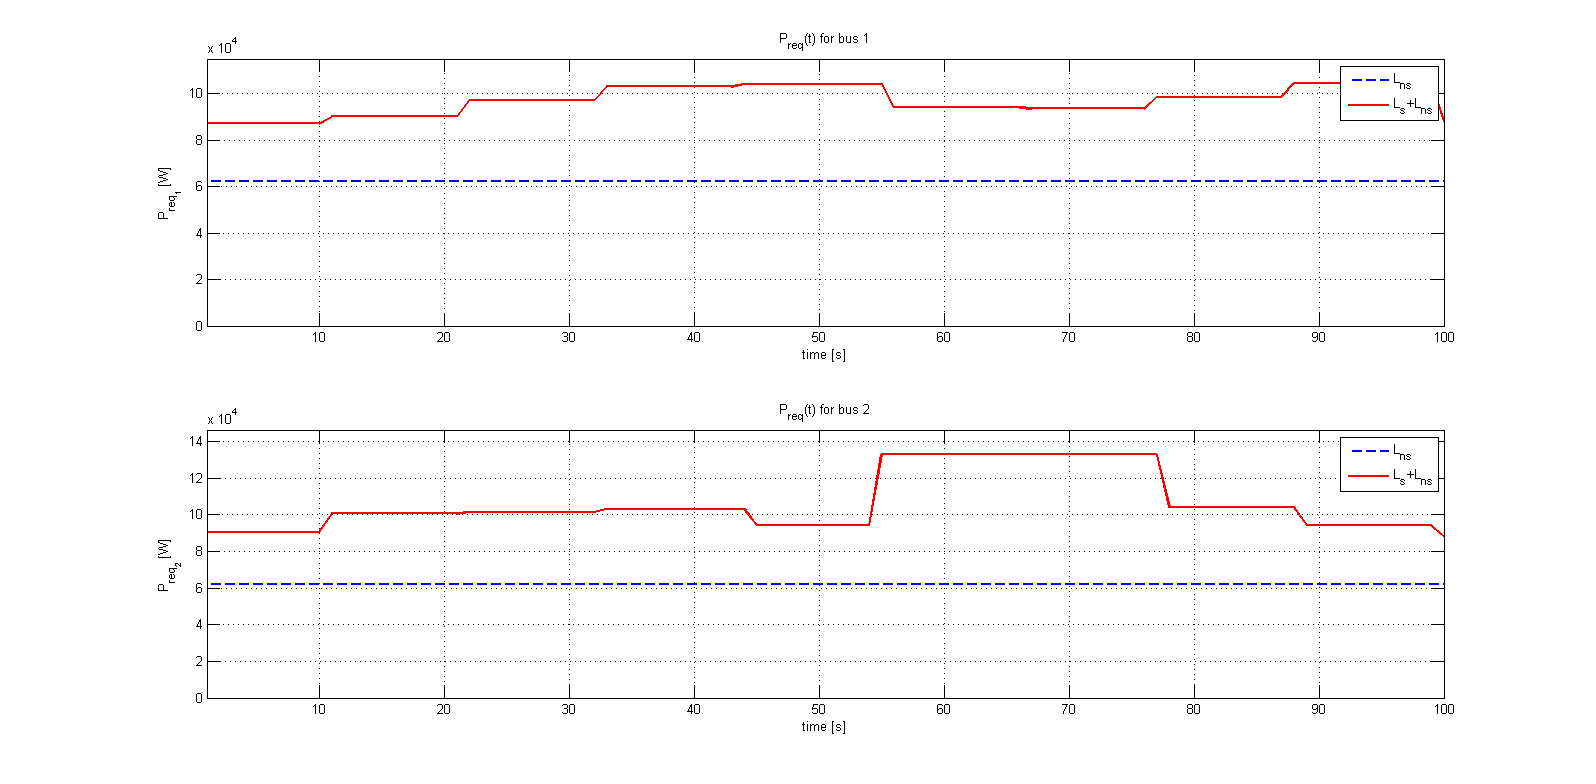
\includegraphics[width=0.9\columnwidth]{figures/preqnofail.png}
  \caption{\textbf{Power Request}
  Historical data of power request on Bus 1 and Bus 2 for time 0
  to 100. Notice the spikes in power usage on Bus 2 that pulls the
  request over 100000 Watts, well over the power rating of the generators.
  Load shedding is a must during those intervals.}
  \label{fig:preqnofail}
\end{figure}

\subsection{No Failures}
\begin{figure}[ht]
  \centering
  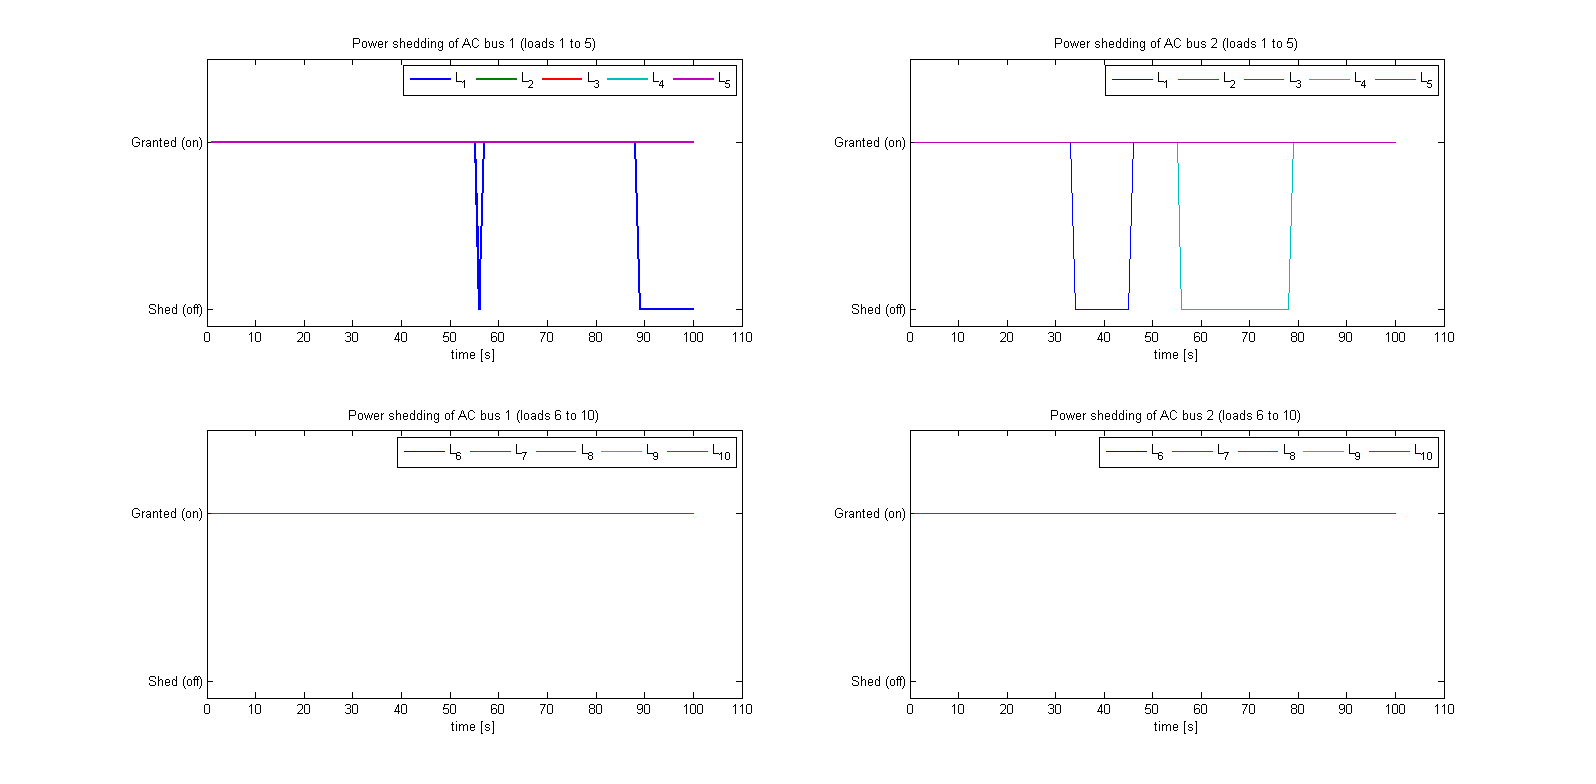
\includegraphics[width=0.9\columnwidth]{figures/lshlnofail.png}
  \caption{\textbf{Optimizing LMS Load Shedding} Notice the long
  period of load shedding around the power usage spikes.}
  \label{fig:lshlnofail}
\end{figure}
\begin{figure}[ht]
  \centering
  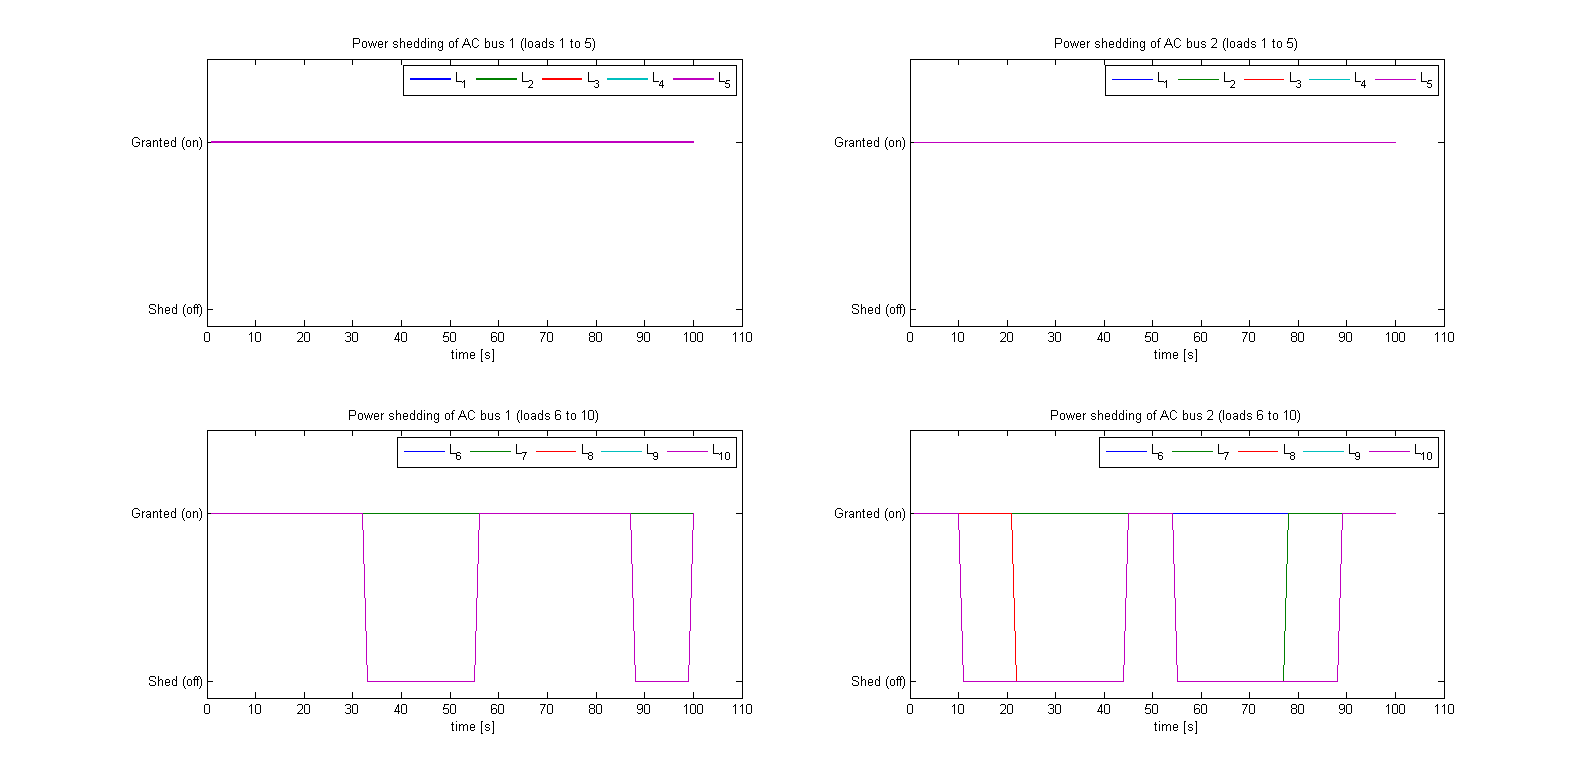
\includegraphics[width=0.9\columnwidth]{figures/lsllnofail.png}
  \caption{\textbf{LL-LMS Load Shedding} Notice that the 
  LL-LMS sheds much more load than the Optimizing LMS.}
  \label{fig:lsllnofail}
\end{figure}

For our first experiment, we simulated the case when there are no power
generator failures in the system using the power usage profile shown in
Figure~\ref{fig:preqnofail}. 
In other words, the real power usage profile (Figure~\ref{fig:preqnofail}) is given to the Optimizing LMS and LL-LMS without any perturbations.
Notice that Bus 1 requests more than 100,000 Watts
between time 30 and 60 and again around time 90. Bus 2, on the other hand,
has a massive power usage between time 50 and 80. We wanted to see how the
Optimizing LMS and the LL-LMS responds to this scenario in isolation. 
%Our results are in Figure~\ref{fig:lshlnofail} and Figure~\ref{fig:lsllnofail}.
Comparing the results, we can see that the LL-LMS will shed a much larger
number of loads (Figure~\ref{fig:lshlnofail}) than the the Optimizing LMS (Figure~\ref{fig:lsllnofail}). 
In particular, the LL-LMS sheds exclusively from loads 6-10 due to the configuration of the priority table.
However, the Optimizing LMS however is much smarter. 
It is able to minimize the number of loads shed by shedding loads much higher up in the priority table.

\subsection{Generator Failure}
Now, we investigate how our Hierarchical LMS system responds to spontaneous generator failures. 
To this end, we
simulated the case when generator 2 would fail at time 45. Obviously, if the Optimizing LMS were
to run in isolation, it would leave the system unpowered from time 45 to 50. 
Figure~\ref{fig:lsllonefail} shows what would happen if the LL-LMS were to run in 
isolation. Starting at time 45, the LL-LMS sees that generator 2 has failed and it has 
switched to using generator 1 to power both buses according to its priority table. In order
to stay under generator 1's power rating, the LL-LMS sheds a large number of loads on the 
second bus. Figure~\ref{fig:lsolonefail} shows what would happen in a combined Optimizing LMS
LL-LMS system. The Optimizing LMS produces advice to be used from time 40 to 50. Unfortunately,
there is no way for the Optimizing LMS's advice to be aware of the failure at time 45. So, while the advice
from time 40 to 44 is optimal and safe, the advice from 45 to 49 is unsafe. The LL-LMS is
able to see this failure at time 45 and kicks in, ignoring the unsafe advice from the Optimizing LMS. This
behavior is observed in Figure~\ref{fig:lsolonefail} where from time 45 to 49, a large
number of loads are shed. Then at time 50, the Optimizing LMS reoptimizes by turning on the APU.
Notice the difference in the number of loads shed onward from time 50 in 
Figure~\ref{fig:lsllonefail} and Figure~\ref{fig:lsolonefail}.

\begin{figure}[ht]
  \centering
  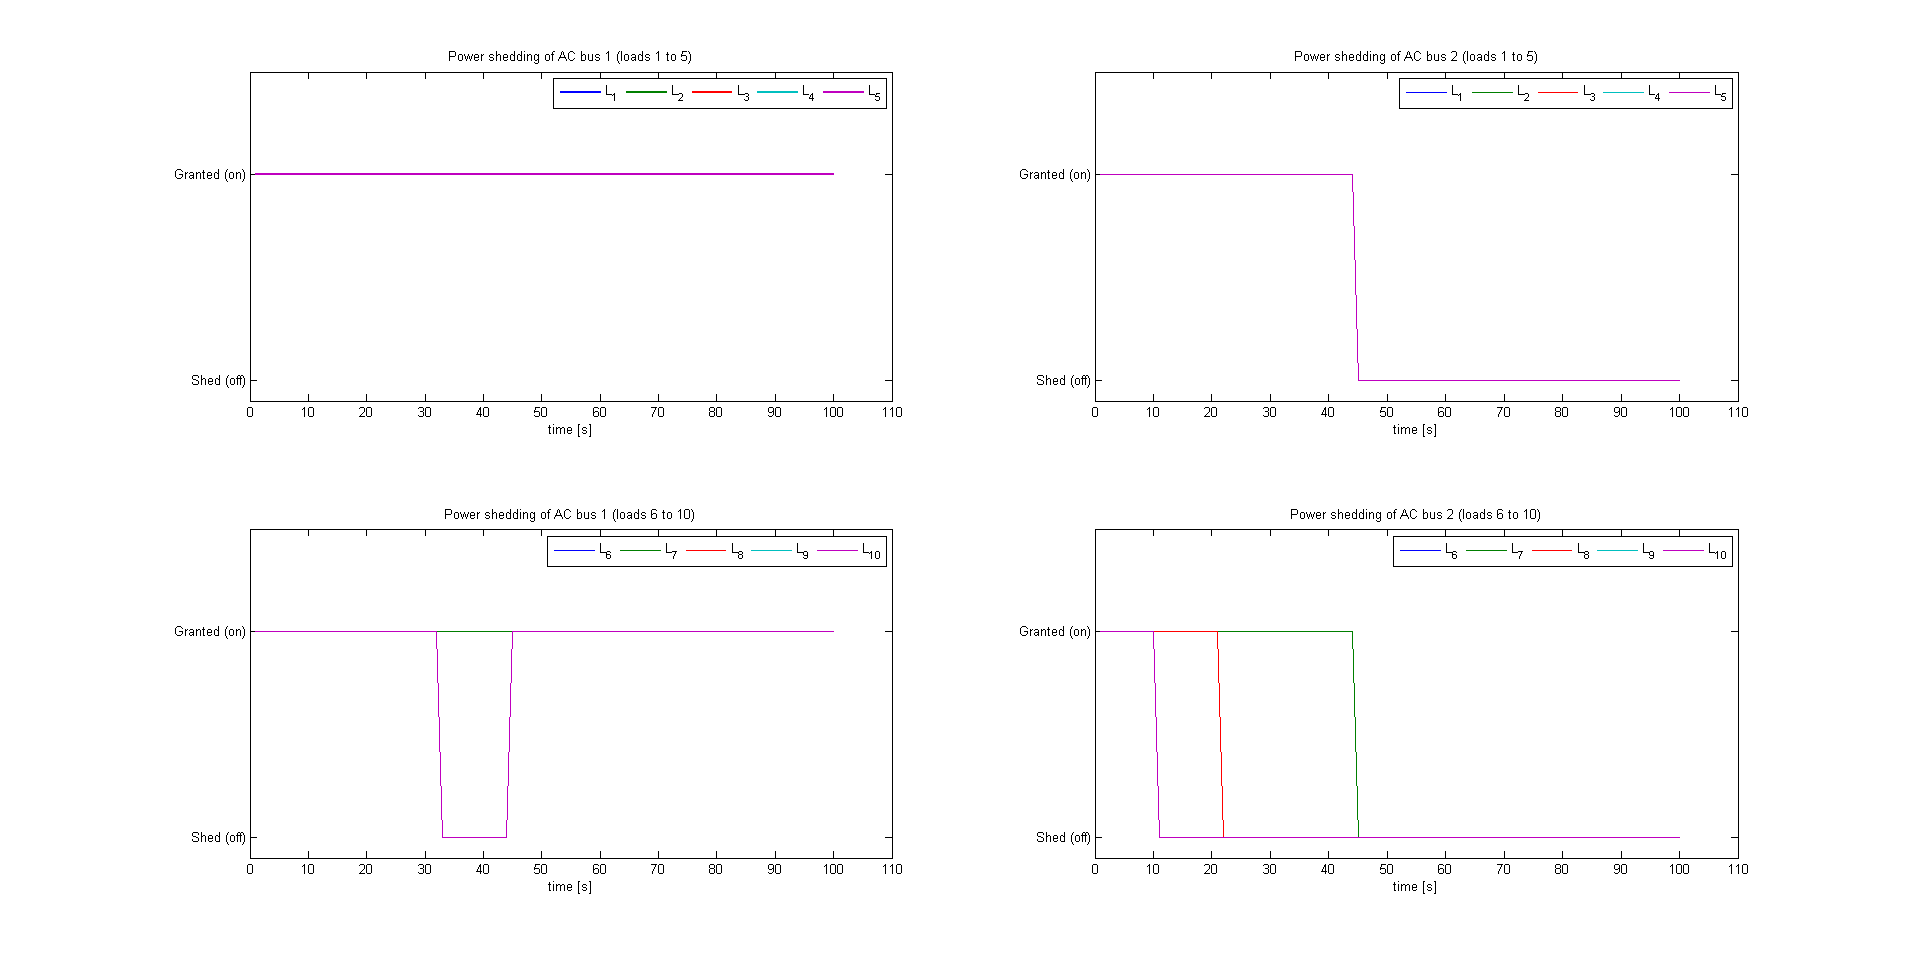
\includegraphics[width=0.9\columnwidth]{figures/lsllonefail.png}
  \caption{\textbf{LL-LMS Load Shedding -- One Failure}. Notice
  the large amount of loads shedded in order to keep power usage below the power rating
  of generator 1.}
  \label{fig:lsllonefail}
\end{figure}
\begin{figure}[ht]
  \centering
  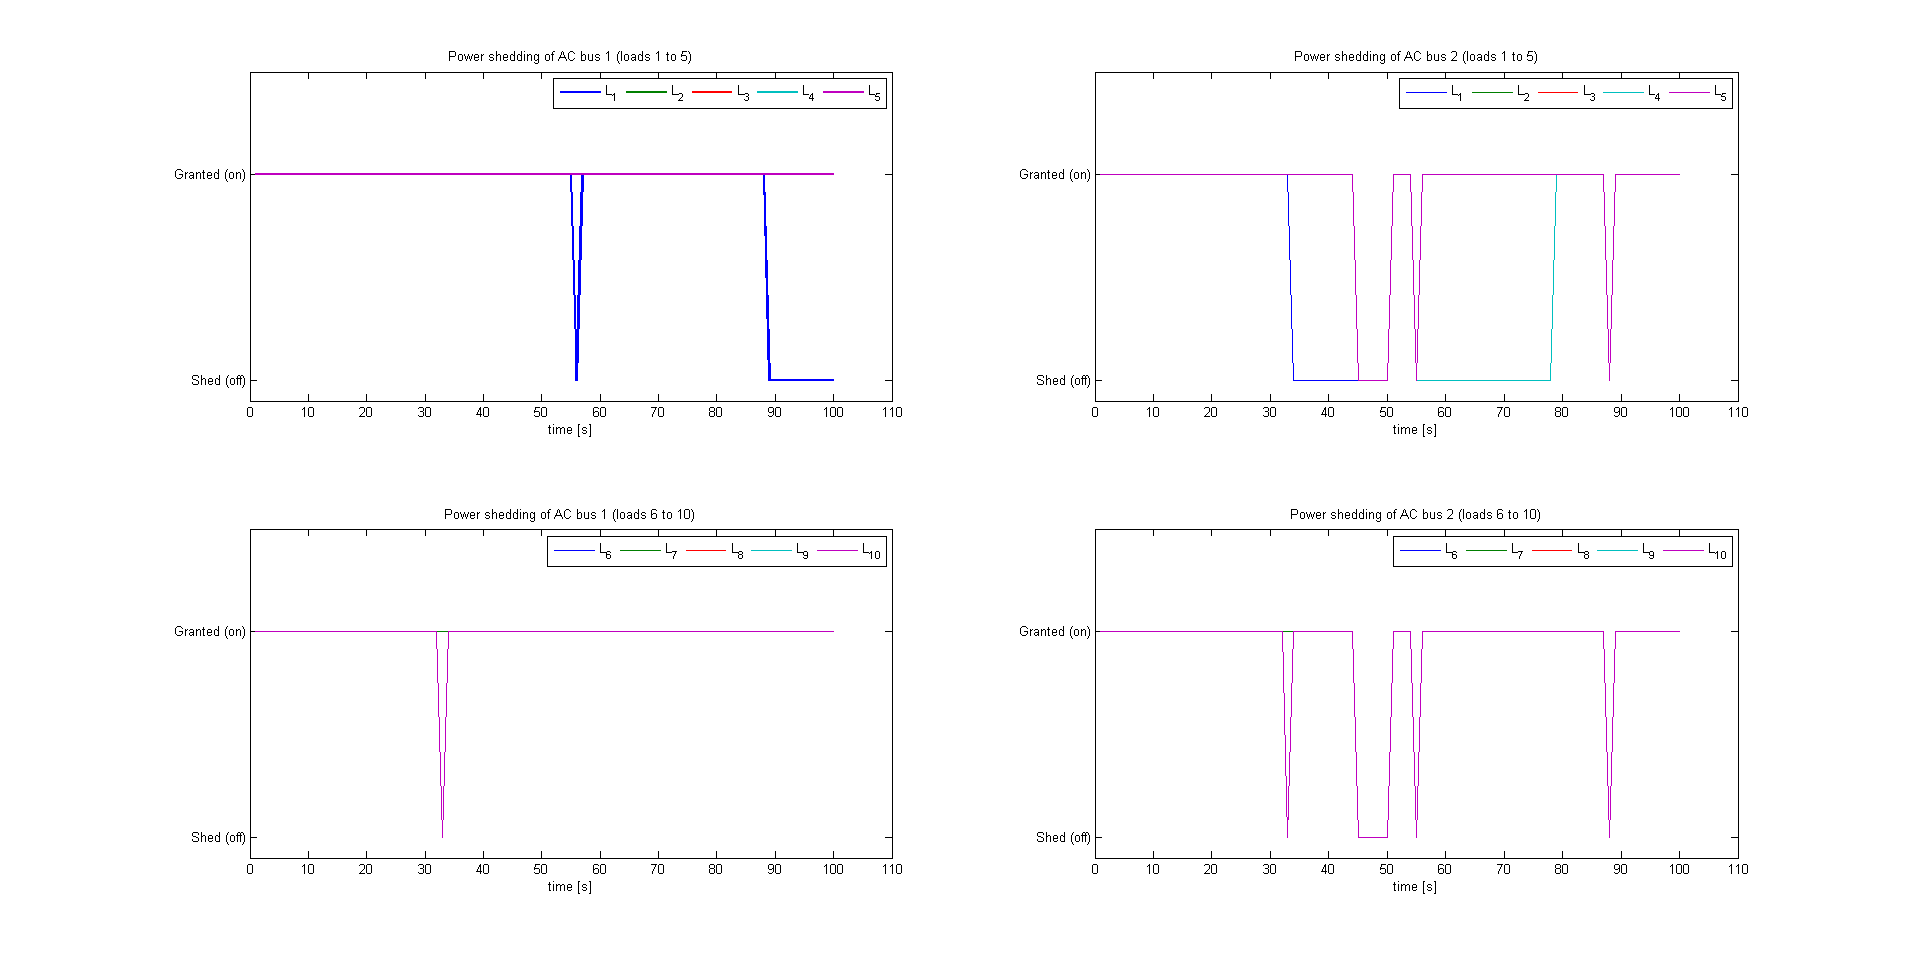
\includegraphics[width=0.9\columnwidth]{figures/lsolonefail.png}
  \caption{\textbf{Hierarchical LMS Load Shedding -- One Failure}. Notice the
  large number of loads dropped from time 45 to 50 before the Optimizing LMS can reoptimize.}
  \label{fig:lsolonefail}
\end{figure}

\subsection{Unexpected Power Spikes}
The Optimizing LMS performs a live optimization using historical data for load power requests from
previous flights. Due to the nature of the optimization problem, it is impossible to
program the optimization problem with live data. As a result, it is possible for the
Optimizing LMS to provide unsafe advice if there is a power spike. More specifically, it is possible
for the Optimizing LMS to generate a load shedding configuration that could have one of the power
generators driving a higher power request than its rating. We want to simulate such a
failure case and show that the LL-LMS performs the required adjustment to keep the system
in a safe state. For this experiment, we use the same historical power request as in
Figure~\ref{fig:preqnofail}. However, the actual power request for this simulation is shown
in Figure~\ref{fig:preqpwrspike}. Without the LL-LMS, the Optimizing LMS would use the load
shedding configuration seen in Figure~\ref{fig:lshlnofail}. Notice that there is a power
spike from time 10 to 40 that the historical data does not account for and thus the Optimizing LMS
is unaware of. As a result, its load shedding configuration would overload the power
generator. Because we have a LL-LMS, we are able to keep the system in a safe configuration.
Figure~\ref{fig:lsolpwrspike} shows that the LL-LMS will detect that the generators would
be overloaded and thus shed some loads during this time interval.

\begin{figure}[ht]
  \centering
  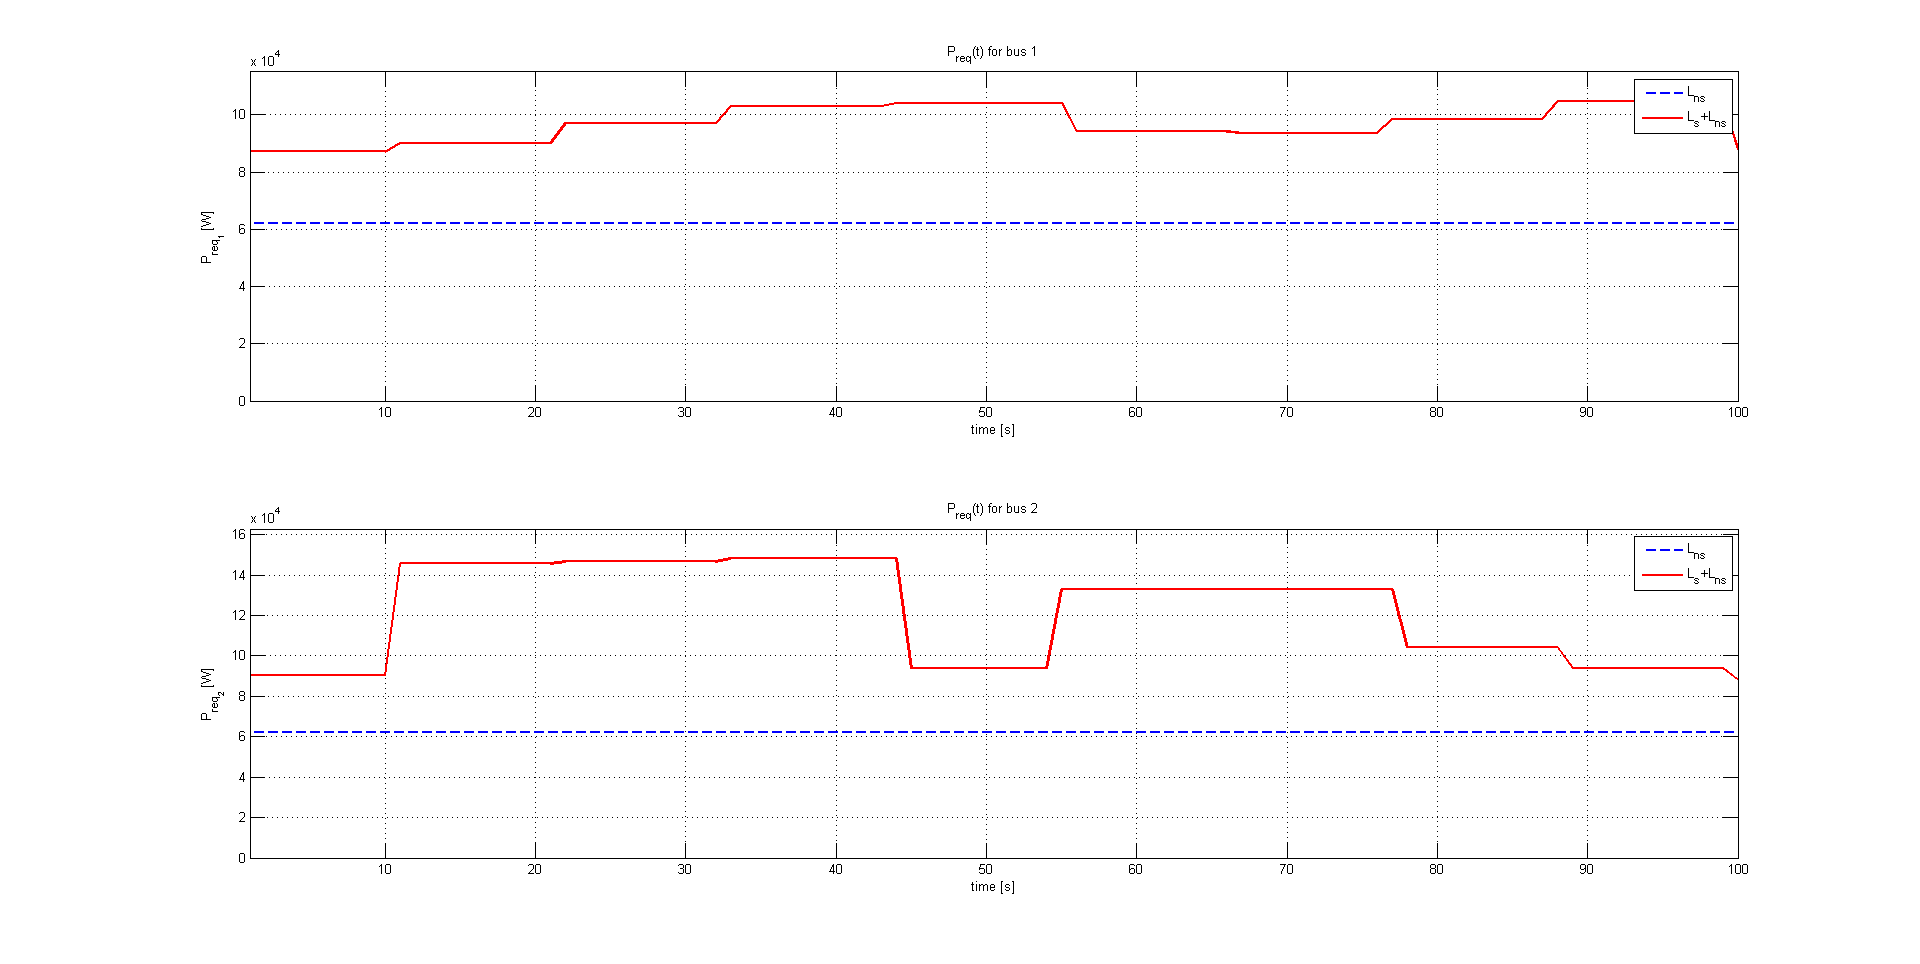
\includegraphics[width=0.9\columnwidth]{figures/preqpwrspike.png}
  \caption{\textbf{Actual Power Request} Notice the difference between this power
  request and the power request expected by the historical data in 
  Figure~\ref{fig:preqnofail}. In particular, there is a large power spike from time 10
  to 40 that is not accounted for in the historical data.}
  \label{fig:preqpwrspike}
\end{figure}
\begin{figure}[ht]
  \centering
  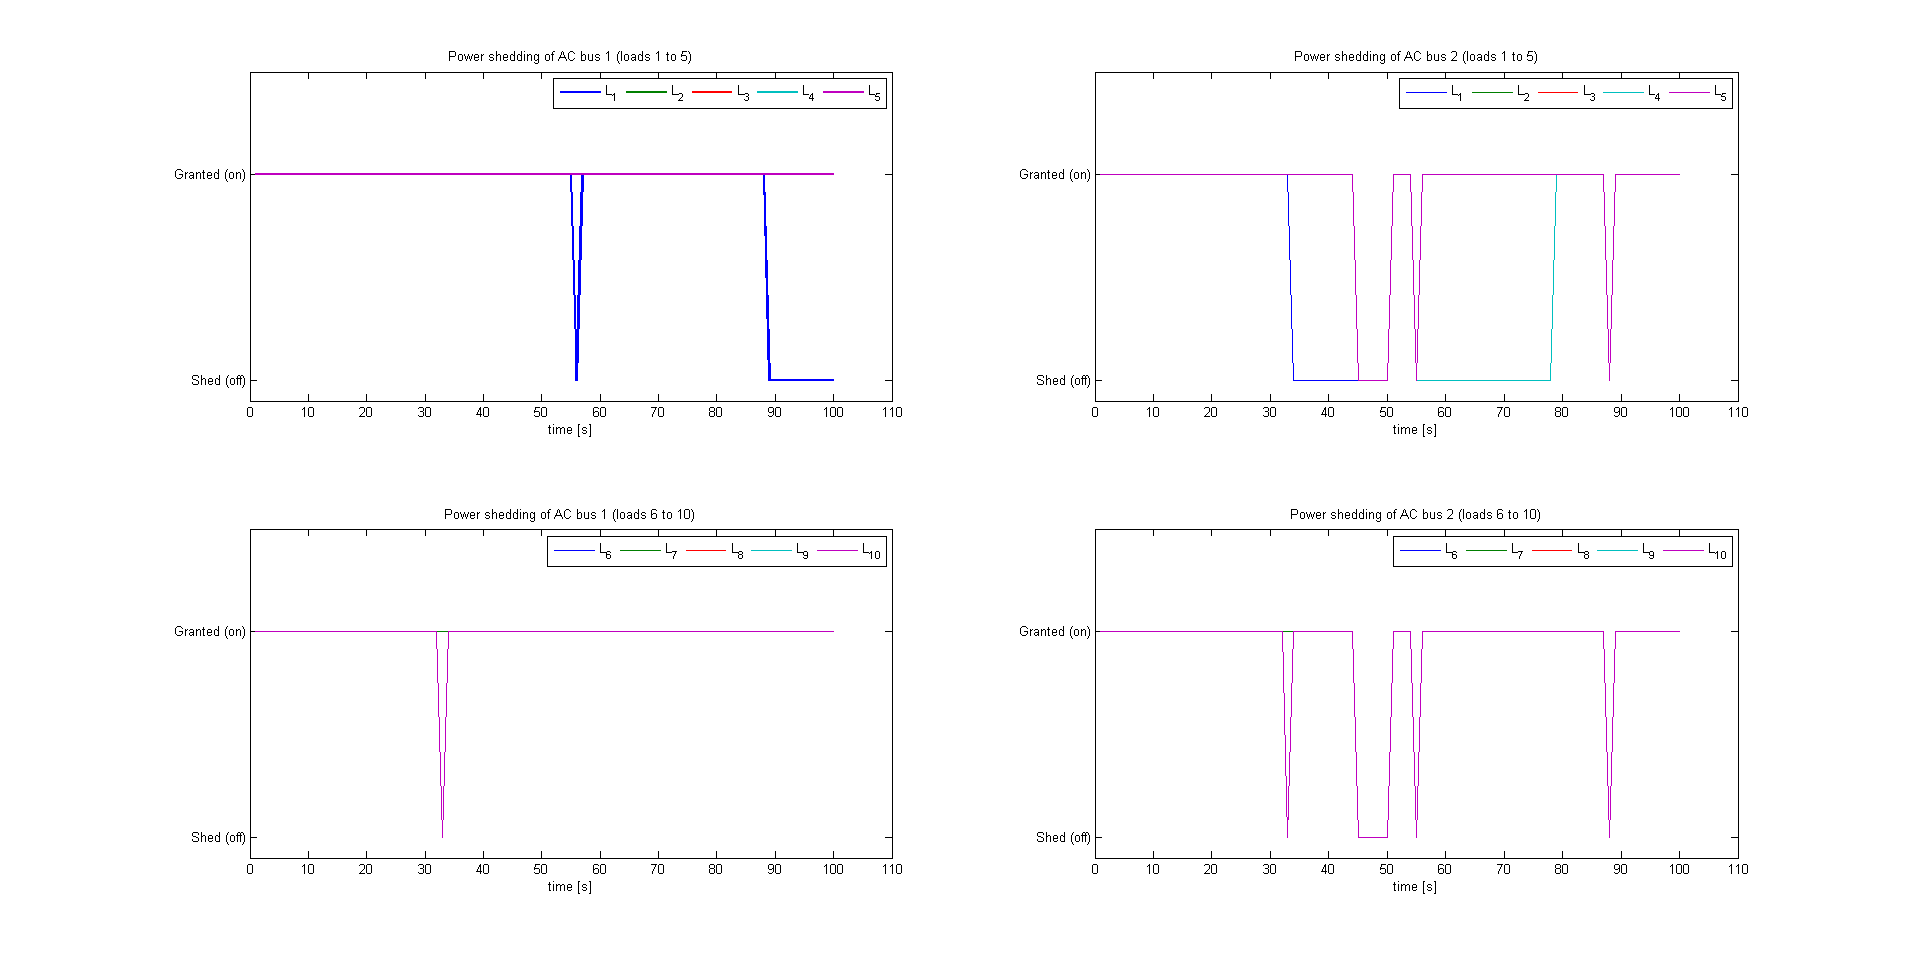
\includegraphics[width=0.9\columnwidth]{figures/lsolonefail.png}
  \caption{\textbf{Hierarchical LMS Load Shedding -- Power Spike} Whenever possible the LL-LMS will
  use the advice from the Optimizing LMS. The only time it ignores the advice from the Optimizing LMS is
  from time 10 to 40 when there is a power spike that the Optimizing LMS is not aware of.}
  \label{fig:lsolpwrspike}
\end{figure}

\section{Conclusion}
Conclusion.

\section*{Acknowledgments}
This work was supported by the US Department of Defense (DoD) through the National Defense Science \& Engineering Graduate Fellowship (NDSEG) Program.

\bibliographystyle{abbrv}
\bibliography{bibliography} 

\end{document}
